		\subsection{GroupBox}

		\begin{frame}
		
		
		\begin{CaixaModelo01}{GroupBox}
			
		O GroupBox permite que sejam agrupados vários controle de forma independente.	

			
		\begin{figure}
				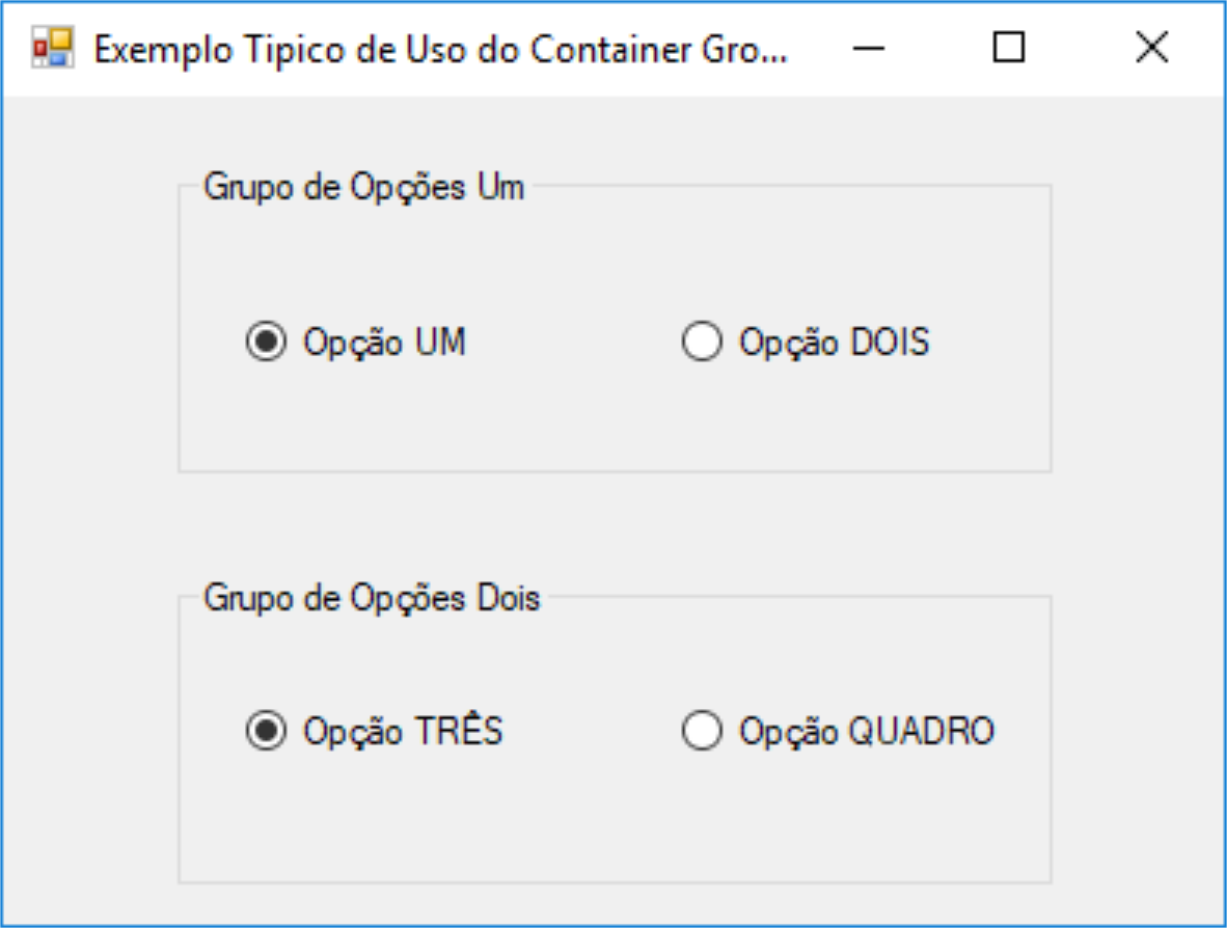
\includegraphics[scale=.6]{./Figuras/F03_GroupBox}
				\caption{Exemplo de uso do GroupBox}
				\label{fig:GroupBox01}
			\end{figure}
			
			
%		\begin{columns}
%			\begin{column}{0.48\textwidth}
%				\begin{figure}
%					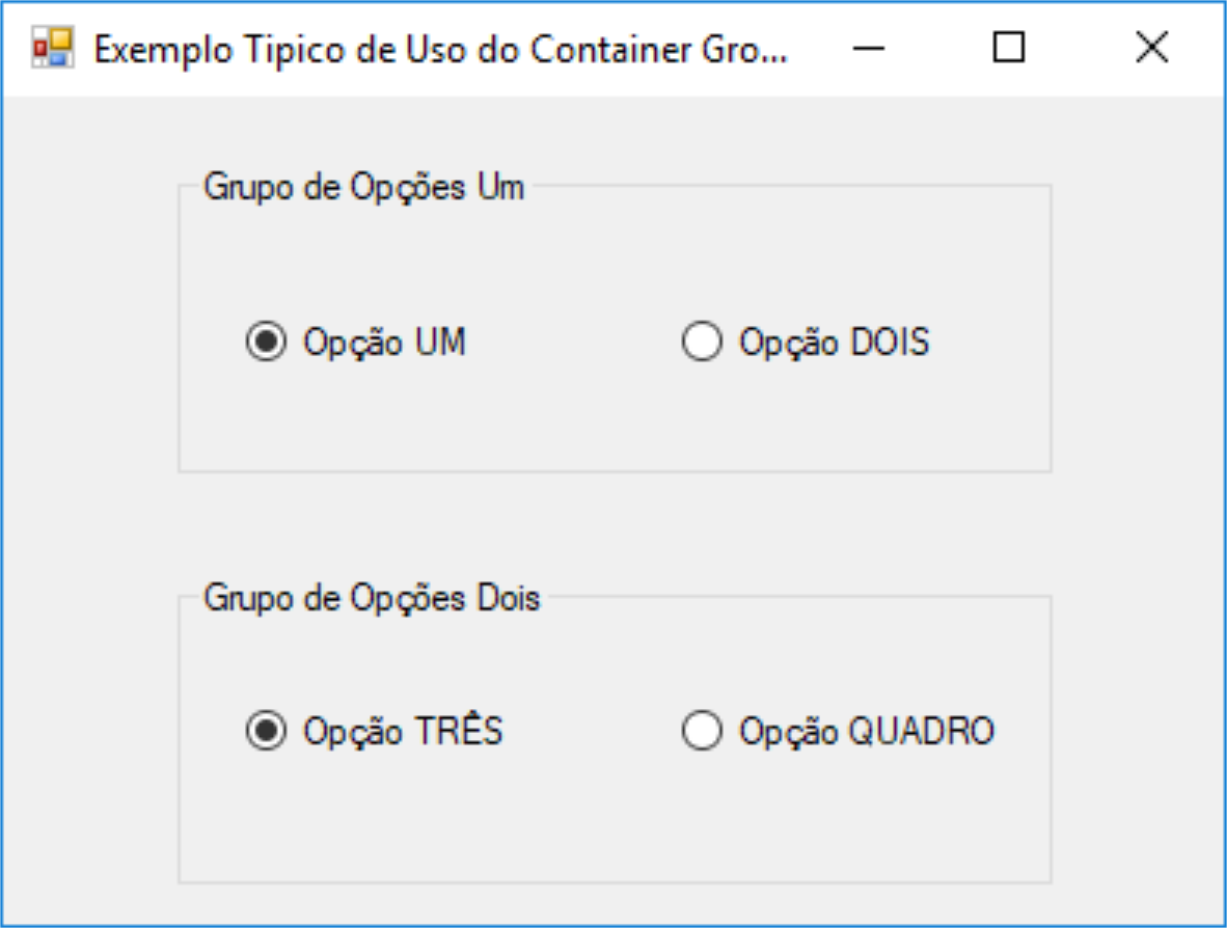
\includegraphics[scale=.4]{./Figuras/F03_GroupBox.png}
%					\caption{RadioButton}
%					\label{fig:RadioButonVerde}
%				\end{figure}
%			\end{column}
%			\begin{column}{0.48\textwidth}
%				\begin{figure}
%					\includegraphics[scale=.4]{./Figuras/RadioButtonVermelho.png}
%					\caption{RadioButton}
%					\label{fig:RadioButonVermelho}
%				\end{figure}
%			\end{column}
%		\end{columns}
		
	   \end{CaixaModelo01}
		

		



		
		
		
%		
%			
%
%	
%		

		\end{frame}